\documentclass{deliverablereport}

\deliverable{dissem}{IntroODK}
\deliverydate{04/09/2019}
\duedate{31/08/2019 (M48)}
\author{Mike Croucher, Hans Fanghor and Nicolas M. Thiéry}

\begin{document}
\maketitle
\enlargethispage{.5cm}
% This will be the abstract, fetched from the github description
\githubissuedescription
\clearpage
\tableofcontents


\section*{Foreword}

Training and dissemination is at the heart of OpenDreamKit; most
participants had been active in this area for a long time before
OpenDreamKit and the project was the occasion to get more resources
for such activities. Sheffield (now Leeds) has been the lead until its
participants got compelling opportunities in the industry in Fall
2018. This did not reduce the overall dissemination activities of the
project: indeed, the freed resources were redistributed to other
participants that were eager to organize more activities than
originally planned. There was some impact however: with continued
leadership some more of the lessons learned at the occasion of those
activities could have been formally collated, when currently many are
in the state of shared folklore. Luckily this information is still
spreading in the community through many channels: informal
discussions, blog posts, mailing lists, etc.

\section{Evaluation and dissemination activities}

As reported on in \delivref{dissem}{workshops-1},
\delivref{dissem}{workshops-3}, and \delivref{dissem}{workshops-4},
OpenDreamKit participants actively organized or participated in 40
events where they advertised and delivered training on OpenDreamKit
technology. We review in this section the other evaluation and
dissemination activities that were carried out during the project.

% \subsection{Dissemination events}

% TODO: Check that this was reported on in the events deliverable and
% remove

% In 2017, we organised a comprehensive workshop on Computational
% Mathematics With Jupyter in Edinburgh, targeting academics, researchers
% and teachers at the same time. Topics delivered by OpenDreamKit members
% included Jupyter, nbdime, nbval, Docker containers, JupyterHub. We
% managed to engage external contributors, such as Christian
% Lawson­Perfect from Newcastle reporting on the Numbas web-based
% e-assessment system for mathematics and Mark Quinn discussing the use of
% SageMathCloud for teaching purposes.

% We contributed a workshop on ``Jupyter Notebooks for reproducible
% research'' at the 2017 International Research Software Engineering
% conference in the UK. While a lot of this work may appear as UK
% -centric, this did have dissemination effects across Europe as the
% emergence of the research software engineering idea and community was
% driven in the UK; researchers across Europe were closely monitored and
% participating in these events.

% K3D-jupyter visualisation widget for
% \Jupyter notebook was presented during PyData Warshaw 2018.


\subsection{Teaching with Jupyter}

Many -- if not most -- of the OpenDreamKit participants engaged
actively in using and testing Jupyter technologies in their daily
teaching duties. Here are some striking examples:

\begin{itemize}
\item At Southampton, OpenDreamKit experts on Jupyter delivered
  multiple courses at the National Centre for Doctoral Training in
  Next Generation Computational Modelling (NGCM), which was the
  occasion to evaluate and disseminate OpenDreamKit technology,
  notably the tools developed there: \longdelivref{UI}{jupyter-test},
  \longdelivref{UI}{jupyter-collab}.

  This included the NGCM Summer School 2016 and 2017 at Southampton,
  which attracted many PhD students and some researchers from the UK,
  Europe and some from overseas.

\item Paris Sud participants used Jupyter in a variety of classes
  (data analysis, programming, computer graphics, graph theory,
  computational combinatorics, computational algebra, experimental
  mathematics, numerical analysis) throughout the math and computer
  science curriculum. An highlight is a 400 students class
  \emph{Introductory programming in C++}. Having a uniform user
  interface across systems (C++, Python, SageMath, \ldots) was a major
  selling point by enabling students to be immediately productive in
  their new environment. The teaching was supported by the deployment
  of a local JupyterHub Virtual Environment and the occasion to
  experiment with various tools including the notebook converters
  nbsphinx and nbconvert, the C++ interactive interpreter xeus-cling,
  Jupyter widgets, interactive web pages with ThebeLab, assignement
  handling and grading with nbgrader. This led to an invitation of the
  course leader to a workshop in Edinburgh to share experience and
  participate to an nbgrader coding sprints where several
  contributions were submitted and accepted.
\item Gent participant introduced SageMath and Jupyter in a variety of
  mathematical courses and engaged other teachers in the process.

\item Since 2017, the University of Versailles uses JupyterLab as the
  working environment for all computational courses in the ``Applied
  Algebra'' Master's program, which enrolls around 50
  students. Through it, the students have access to the Jupyter
  notebook, a Unix shell (Bash), and tools to code in C, Python,
  SageMath, and many more languages.

  This JupyterHub based Virtual Environment deployment has been described in detail on
  the OpenDreamKit
  blog\footnote{\url{https://opendreamkit.org/2018/10/17/jupyterhub-docker/}};
  the associated GitHub
  repository\footnote{\url{https://github.com/defeo/jupyterhub-docker}}
  has been \emph{starred} 47 times, \emph{forked} 33 times, and the
  author regularly receives requests for help, showing that there is a
  growing interest in deploying similar setups at other universities
  and research centers.

  The VRE has been opened in 2019 to the whole university, with an
  expanded set of tools. In the upcoming academic years other programs
  will start using it for their courses.
\item
  The University of Silesia uses elements of \ODK in many aspects of
  education. JupyterHub is installed on the campus facilities and it
  is available for students. Currently there are c.a. 1000
  users. There is an experimental setup for research backed by slurm
  HPC cluster and jupyter-batchspawner. There are courses for physics
  and biophysics students which are using interactive books produced
  during \ODK. Data science oriented courses (Introduction to AI and
  Machine Lerning) are fully based on \Jupyter and nbgrader system for
  distribution and collection and grading of excercises. Courses in
  \Python programming for computer science students are using \Jupyter
  notebook. There are experimental attempts to use IJava kernel with
  \Jupyter for introductory Java course. \SageMath is presented to
  students of physics and biophysics during first course in ICT and
  then used during whole course. 
\item
  In USTAN, Alexander Konovalov introduced Jupyter notebooks
  for teaching Python in the 2nd year module. Lecture materials 
  were provided in the form of Jupyter notebooks, which both lecturer
  and students were able to execute during the lecture. One of the
  course practicals consisted of producing a reproducible report
  about analysing a dataset, which had to be submitted in the form
  of a Jupyter notebook. Furthermore, Konovalov demonstrated the usage
  of Jupyter notebooks for sharing reproducible computational 
  experiments using Microsoft Azure and Binder in a number of 
  workshops for USTAN staff and research students.
\item
  Sheffield OpenDreamKit participants spearheaded a transformation in
  the way computation was taught at The University of Sheffield across
  multiple subjects and at many levels. The Department of Physics, for
  example, now teaches \emph{all} of its undergraduates how to program
  in Python using Jupyter notebooks and the CoCalc (Formerly
  SageMathCloud) cloud-based environemnt. Furthermore, many other
  physics modules at Sheffield now include some type of computation
  using the same technologies. Programming is no longer considered
  separately but as the integral part of modern science that it really
  is.

  Working with an Italian Marie-Curie fellow in Bioinformatics,
  Sheffield's OpenDreamKit participants developed a set of short
  postgraduate `Bioinformatics Awareness Days' which used OpenDreamKit
  technology to introduce Bioinformatics workflows to clinicians at
  Sheffield's Institute for Translational Neuroscience. This further led
  to an OpenDreamKit teaching tutorial being held at University of
  Naples Parthenope.

  Other subject areas where Sheffield's OpenDreamKit participants
  assisted in developing enhanced lecture material using OpenDreamKit
  technologies include Machine Learning, Mathematics, Computer Science,
  Biology and High Performance Computing.
\end{itemize}

\subsection{Teaching material}

Interactive lecture notes are an area where commercial vendors such as
MapleSoft and Wolfram Research are spending a lot of time and money
developing material. Within the Jupyter ecosystem it has become possible
to author interactive lecture notes and make them openly available
(e.g.~through BinderHub). We have created such interactive lecture
materials, used them in university education, and made them openly
available on the Internet. This includes four interactive textbooks (see
\longdelivref{dissem}{ibook1} and \longdelivref{dissem}{ibook3c}), but also Software Carpentry lessons, course notes,
etc.

Anecdotal evidence and feedback from individual users (see D2.14) shows
that they are used outside the OpenDreamKit partners, in and out of
Europe, both by individual students and university lectures.

\subsection{Local consulting}

Across all the OpenDreamKit partner sites, OpenDreamKit staff and PIs
have engaged with colleagues, students and decision makers to advocate
the benefits of the Jupyter research environment; often effectively
serving as consultants for best practice computational mathematics and
science tools and workflows.

For example,
at Sheffield, a taster seminar (1-2 hours) and follow-up short course (1-2
days) on Jupyter for lecturers and researcher were organised targeting
and engaging science and engineering disciplines beyond mathematics as
the Jupyter ecosystem of tools is of value for teaching and research in
any discipline having to work with computational and data based
research. These workshops were integrated into the research support
services of the Sheffield IT department, and integrated with the
research software engineering movement that originated in the UK over
the previous years.

The OpenDreamKit funding was essential in forming Sheffield's Research
Software Engineering (RSE) Group, one of the first such groups in the
UK. Providing training, documentation and support in the use of
OpenDreamKit technologies in both teaching and research helped the
Sheffield RSE group demonstrate to the University how vital RSE support
can be. This directly led to the fully-funded, diverse group that now
exists at Sheffield which has served as a model for many other such
groups around the UK, Europe and more, recently, the United States.
This was documented in our blog post
\href{https://opendreamkit.org/2018/10/29/ODK-RSE/}{\emph{How OpenDreamKit
  supported the RSE revolution}}.

\subsection{Contributions}



\begin{itemize}
\tightlist
\item
  Tania's course template
\item
  Marcin's bookbook cookie-cutter
\end{itemize}

\section{Evaluation and adoption}

By design, the target audience for this project is extremely diverse,
and the toolkit approach makes it so that there isn't such a thing as
a well defined end-product of OpenDreamKit. Hence trying to capture
the adequateness and the adoption through, e.g., polls or metrics
makes limited sense. Instead, we focused on gathering feedback through
first hand experience, and continuous contacts with a large variety of
end-users during all the activities reported on above.

To give a sense of the lessons learned, we reflect in this section on
how some of the tools we have promoted appeared adequate for the users
needs and adopted by the community.

\subsubsection{The Jupyter notebook}

Based on our dissemination activities, the Jupyter notebook is
emerging as one of the major user interfaces for computational (pure)
mathematics, if not the de-facto standard in many communities. A key
selling point is having a uniform interface across computational
tools, thanks notably to \longdelivref{UI}{ipython-kernels}.

This is in line with the general evolution in areas such as scientific
computing and data sciences. As anecdotal evidence, the use of
notebooks at Sheffield, Southampton, XFEL and other universities has
grown significantly. Also, the integration of Sun Grid Engine and
Project Jupyter, done as part of OpenDreamKit
(\delivref{hpc}{SGE-jupyter}), has led to educators using the
notebook to introduce various aspects of High Performance Computing.

We now detail two typical lessons we have learned.

Practice over hundreds of students in class or other learners at
dissemination workshops have shown that it takes no more than an hour of
guided instruction to become sufficiently acquainted with the basics of
the Jupyter notebook to be able to autonomously explore properly
structured collections of notebooks (e.g.~an interactive text-book, or a
collection of tutorials in a workshop). At this stage, the simple,
linear narrative structure of a notebook is a precious guide to the
reader.
It does take some practice however for the user to not get any more
confused by the potential disprecancy between the visual order and
execution order of cells. This can be mitigated by short notebooks, and
the use of notebook extensions that enforce the execution order of
cells.

Properly authoring one's own notebooks also takes a lot of practice.
The simplicity of incrementally building code by testing code snippets
and aggregating them is a big strengh of the notebook. It's also a
weakness: notebooks have a tendency to grow organically and become
bloated and unstructured. This natural tendency must be explicitly
counteracted upon through training and the sharing of best practices.

\subsubsection{Jupyter widgets}

Among the technologies we disseminate, Jupyter widgets are one with
the largest ``Wow'' factor, sparking ideas among our users on how they
could be exploited for, e.g., teaching or research. As we anticipated,
the learning curve remains steep however. Most users stay at the basic
stage of authoring so-called interacts. Few actually take advantage of
the full flexibility offered by widgets to build interactive
applications by combination thereof. Authoring one's own completely
new widget (e.g. for a new type of visualization) takes specific
expertise, notably to implement the Javascript side of it. One
strategy to tackle this is to have Research Software Engineer leverage
the technology to non experts by implementing generic widgets that can
be specialized to cover a range of use cases. This approach was
validated at the occasion of two of our dissemination events at CIRM \href{https://conferences.cirm-math.fr/1978.html}{\emph{Free Computational Mathematics}}
and Ljubljana \href{https://wiki.sagemath.org/fpsac19}{\emph{SageDays 105}} where the generic widgets of
\longdelivref{UI}{ipython-advanced-interacts} were presented, and then
adopted and extended by several PhD students.

Here is such an \href{https://github.com/nheir/sage-combinat-widgets/blob/example_parapolyomino/examples/ParalleloPolyomino.ipynb}{\emph{example notebook for a Parallelogram Polyomino}} with following resulting \emph{interactive widget} (see figure next page .. FIXME)

\begin{figure}[ht]
  \caption*{A Parallelogram Polyomino.}
  \medskip
  \small{Clicking on corners increase/decrease polyomino \emph{size}, while polyomino \emph{unicode} representation and \emph{Dyck word} are displayed in real time.}
\resizebox{160mm}{!}{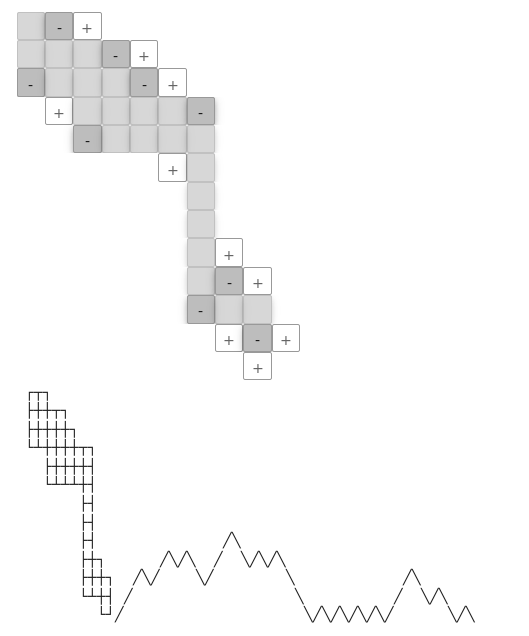
\includegraphics{nheir_parallelogram_polyomino.png}}
\end{figure}

\subsubsection{3D visualization}

\subsubsection{Computational systems}

\subsubsection{Notebook validation and version control with nbval and nbdime}

Our development and dissemination activities on \nbval and \nbdime
(\delivref{UI}{jupyter-test}, \delivref{UI}{jupyter-collab}) within
OpenDreamKit has resulted in researchers switching to using the
notebook for all of their software documentation and tutorials. They
also confirmed in practice the unique selling point of \nbval:
ensuring that notebook-based documents stay up to date and functional
even as the underlying software stack and environment evolves. In
particular, \nbval allows notebook-based documentation to become part
of the formal testing and continuous integration framework.

\subsubsection{Interactive documents}

We refer here to Section 4 of \longdelivref{dissem}{ibook3c}.

\subsubsection{Class management}

There are various methods for managing classes using OpenDreamKit
technologies and OpenDreamKit participants have tried most of them. None
of them are perfect and many non-specialist lecturers require support in
choosing and using the various options which include:

\begin{itemize}
\tightlist
\item Commercial Cloud-based environments such as Microsoft Azure,
  Google's Collab and CoCalc. These are very easy to set up and use.
  The main caveat is the loss of control, notably in term of private
  data protection. Practical issues included updates occuring in the middle of exam
  sessions that modified user-interface behaviour and even computational
  results in some cases. For one computationally intense course, the
  amount of CPU power available in the cloud environment was
  insufficient for students to complete some project work which led to
  complications.
\item
  Bring your own laptop. Such sessions ensure that participants leave
  teaching sessions with a fully functioning computational environment
  but supporting diverse operating systems and hardware can be extremely
  challenging for those running the course.
\item Server or computer lab run by University IT. They can provide a
  very controlled and stable environment but at the cost of teachers
  not being able to update in a timely fashion unless the servers are
  supported by dedicated Research Software Engineering staff.
\item Server or software environment in the computer lab setup by the
  teacher. This is the most flexible solution, but requires strong
  computer literacy, and also the agreement of the University IT. The main
  difficulty is the integration with the local information system.
\end{itemize}

When using this type of technology across many subjects in a
University, it quickly becomes apparent that, at this stage, the only
way to fully support lecturers properly is to have on-site specialists
that can provide the required assistance. Such work forms the
foundation of the Research Software Engineering groups that have
started to form all over the world. OpenDreamKit participants formed
the first demonstrations of such partnerships

On the technical side, one of the most popular tool for managing
assignments in a class is nbgrader; it supports authoring,
production and distribution of instructor and student version,
collection, semi-automatic grading, feedback. It is modular and each
piece can be used either from a graphical user interface (UI) within
Jupyter or from the commandline. This gives, in principle, quite some
flexibility to integrate it into the local information system and
workflow.

Experience shows that usage through the UI is straightforward, for
students and instructors alike, even novices. However, as of now,
setting it up requires good computer literacy, if not admin right on the
local system. The tricky part is to setup the \emph{exchange zone}
through which assignments are exchanged back and forth between
instructor and students. Support for multiple courses and
multi-instructor courses is also very recent. We expect the entry
barrier to decrease greatly with the ongoing development of an
\emph{exchange service}; once deployed locally at an institution and
integrated with the local information system, instructors will be able
to seamlessly setup new courses.

\subsubsection{Packaging and distribution}

See \delivref{component-architecture}{sage-distribution}.

\subsubsection{Binder}

\subsubsection{VRE access / deployment}

\subsubsection{Integration with EOSC}

All technologies developed in OpenDreamKit is based on open, standard,
and modern web technologies, which should make it straightforward to
integrate in larger infrastructure or infrastructure federation, and
notably the European Open Science Cloud. This claim is well supported
by two major instances: first, a JupyterHub service was deployed in
2017 by EGI as a service for the EOSC, and has been running
continuously since then; second, 


% \subsection{Reflection about ``small contributions'' making large  impact}

% was it efficient?

% \begin{itemize}
% \tightlist
% \item
%   feedback loop
% \item
%   not easy to fund
% \item
%   not easy to find people who want to do this
% \item
%   the value of what we disseminated was for many participants dominated
%   by learning about the basics of the tools rather than the more
%   advanced extensions implemented through OpenDreamKit
% \end{itemize}

%\section{Stuff that could be added}

\end{document}

%%% Local Variables:
%%% mode: latex
%%% TeX-master: t
%%% End:

